% Per-triangle UE-anchored Kirchhoff render schematic, for JSAC2 §IV
\documentclass[border=4pt,tikz]{standalone}
\usepackage{amsmath,amssymb}
\usepackage{bm}
\usepackage[T1]{fontenc}
\usepackage{lmodern}
\usepackage{tikz}
\usetikzlibrary{positioning,arrows.meta,calc,decorations.markings}

\definecolor{netblue}{HTML}{1F4E79}
\definecolor{twinorange}{HTML}{B26A00}
\definecolor{usergreen}{HTML}{2E7D32}
\definecolor{rayred}{HTML}{C42E2E}

\begin{document}

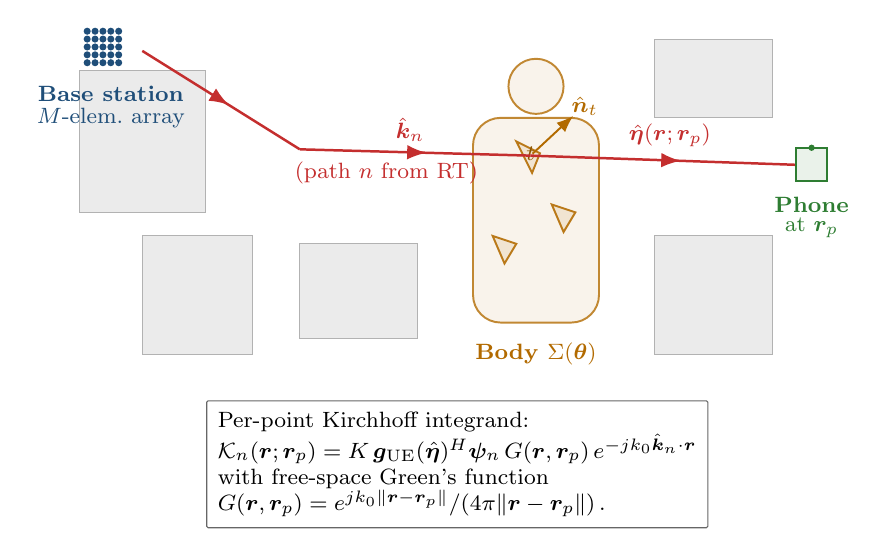
\begin{tikzpicture}[
    every node/.style={font=\small},
    arrow/.style={->, line width=0.7pt, >=Latex, shorten >=1pt, shorten <=1pt},
    ray/.style={line width=0.9pt, color=rayred, postaction={decorate},
                decoration={markings, mark=at position 0.55 with {\arrow{Latex}}}},
    triangle/.style={draw=twinorange!90, line width=0.7pt, fill=twinorange!18},
    building/.style={draw=black!30, line width=0.4pt, fill=black!8},
]

% --- Environment: a couple of buildings sketched as light grey blocks
%     (suggests urban canyon: BS sits above scene, paths route via
%     building reflections + LOS to the body) ---
\fill[building] (-5.8, -0.2) rectangle (-4.2, 1.6);
\fill[building] (-5.0, -2.0) rectangle (-3.6, -0.5);
\fill[building] (-3.0, -1.8) rectangle (-1.5, -0.6);
\fill[building] (1.5, -2.0) rectangle (3.0, -0.5);
\fill[building] (1.5, 1.0) rectangle (3.0, 2.0);

% --- Base station: 5x5 dots, mounted on a tall building edge ---
\foreach \i in {0,...,4}{
  \foreach \j in {0,...,4}{
    \fill[netblue] (-5.7 + 0.10*\i, 1.7 + 0.10*\j) circle (0.045);
  }
}
\node[netblue, font=\footnotesize\bfseries, align=center]
     at (-5.4, 1.3) {Base station};
\node[netblue, font=\footnotesize, align=center]
     at (-5.4, 1.0) {$M$-elem.\ array};

% --- Body silhouette: head circle + torso rounded rectangle ---
\draw[draw=twinorange!80, line width=0.7pt, fill=twinorange!8]
  (0, 1.4) circle (0.35);
\draw[draw=twinorange!80, line width=0.7pt, fill=twinorange!8,
      rounded corners=10pt]
  (-0.8, -1.6) rectangle (0.8, 1.0);
\node[twinorange, font=\footnotesize\bfseries, align=center]
     at (0, -2.0) {Body $\Sigma(\bm{\theta})$};

% --- Highlight one triangle ($t$) and a couple of context triangles ---
% Main triangle on the chest, near (-0.05, 0.5)
\draw[triangle] (-0.25, 0.7) -- (0.05, 0.55) -- (-0.05, 0.30) -- cycle;
\node[font=\footnotesize, color=twinorange!80!black] at (-0.07, 0.55) {$t$};
% Context triangle on the lower torso
\draw[triangle] (-0.55, -0.5) -- (-0.25, -0.6) -- (-0.40, -0.85) -- cycle;
% Context triangle on the abdomen
\draw[triangle] (0.20, -0.1) -- (0.50, -0.2) -- (0.35, -0.45) -- cycle;

% --- Outward normal at triangle t ---
\draw[arrow, color=twinorange, line width=0.7pt]
   (-0.07, 0.52) -- (0.50, 1.05);
\node[font=\footnotesize, color=twinorange] at (0.62, 1.15) {$\hat{\bm{n}}_t$};

% --- Incident path from BS to triangle t (via a building edge to suggest
%     scene multipath, not just LOS) ---
\draw[ray] (-5.0, 1.85) -- (-3.0, 0.6);                  % BS -> building edge
\draw[ray] (-3.0, 0.6)  -- (-0.07, 0.52);                 % edge -> triangle t
\node[rayred, font=\footnotesize] at (-1.6, 0.85) {$\hat{\bm{k}}_n$};
\node[rayred, font=\footnotesize]       at (-1.9, 0.30) {(path $n$ from RT)};

% --- Reflected ray from triangle t to phone ---
\draw[ray] (-0.07, 0.52) -- (3.4, 0.40);
\node[rayred, font=\footnotesize] at (1.7, 0.78) {$\hat{\bm{\eta}}(\bm{r};\bm{r}_p)$};

% --- Phone at right ---
\draw[draw=usergreen, line width=0.7pt, fill=usergreen!10]
  (3.3, 0.20) rectangle (3.7, 0.62);
\fill[usergreen] (3.5, 0.62) circle (0.04);
\node[usergreen, font=\footnotesize\bfseries, align=center]
     at (3.5, -0.1) {Phone};
\node[usergreen, font=\footnotesize, align=center]
     at (3.5, -0.4) {at $\bm{r}_p$};

% --- Per-point integrand box, anchored bottom of figure (clear of bldgs) ---
\node[draw=black!60, line width=0.4pt, rectangle, rounded corners=0.5pt,
      inner sep=4pt, fill=white, align=left, font=\footnotesize]
     at (-1.0, -3.4)
     {Per-point Kirchhoff integrand:\\
      $\mathcal{K}_n(\bm{r};\bm{r}_p)
       = K\,\bm{g}_{\mathrm{UE}}(\hat{\bm{\eta}})^{H}\bm{\psi}_n
        \,G(\bm{r},\bm{r}_p)\,e^{-j k_0 \hat{\bm{k}}_n\cdot\bm{r}}$\\
      with free-space Green's function\\
      $G(\bm{r},\bm{r}_p)
       = e^{j k_0 \|\bm{r}-\bm{r}_p\|} / (4\pi \|\bm{r}-\bm{r}_p\|)$\,.};

\end{tikzpicture}

\end{document}
